\parindent=0em
\subsection{Industria}
\noindent

%https://news.microsoft.com/es-es/2019/06/18/airbus-vuela-mas-alto-con-ayuda-de-la-tecnologia-de-realidad-mixta-de-microsoft/

%https://marquesme.com/5-beneficios-clave-de-realidad-mixta-para-la-industria/

Otro ámbito que es potenciado por la realidad mixta es la industria, esta tecnología beneficia a este sector de las siguientes formas:

\begin{itemize}
    \item \textbf{Proceso de control de calidad más rápido:} Estos largos procesos de control de calidad se ven reducidos notablemente haciendo uso de imágenes, textos o modelos 3D en aquellas líneas de producción. Esto da lugar a ensamblajes más rápidos y con menos errores.
    
     \item \textbf{Mantenimientos más rápidos:} Cascos como las \textit{HoloLens2} de \textit{Microsoft} permiten sustituir manuales de reparación tediosos por simples instrucciones en el entorno de realidad mixta. Otro uso para agilizar el mantenimiento es el que hace la empresa de ascensores \textit{ThyssenKrupp} donde sus empleados, haciendo uso de estos cascos de realidad mixta, realizan llamadas al soporte técnico que les guía con facilidad gracias a poder ver en tiempo real el ascensor a través de la retransmisión que ofrecen las gafas.
     
     \item \textbf{Formación de empleados más eficiente:} Cualquier formación puede ser remplazada por un entorno en realidad mixta de situaciones reales o instrucciones con el mundo real frente a los empleados, lo cual hace que al enfrentarse a estas situaciones reales (no como lo harían sin esta tecnología, solo con casos teóricos) ganen aptitudes de una manera más rápida.
     
     \item \textbf{Aumentar la mano de obra cualificada:} Los trabajadores formados mediante realidad mixta pueden durar para siempre, es decir, aunque se jubilen podrían seguir aportando conocimiento (formando o trabajando) de forma remota desde sus casas a través de los dispositivos de realidad mixta.
     
    \item \textbf{Competitividad en el sector:} Todos los puntos anteriores fomentan el crecimiento de la empresa en forma de automatizar procesos, minimizar tiempos y reducir costes, es por esto que el uso de dicha tecnología es necesaria para ser competitivos.
\end{itemize}

La empresa de diseño, fabricación y venta de aviones civiles \textit{Airbus} es una de las beneficiadas por la realidad mixta, esta empresa tardó 40 años en fabricar sus primeros 10.000 aviones, en cambio, haciendo uso de esta tecnología aspiran a fabricar 20.000 aviones más. El vicepresidente ejecutivo de Ingeniería de Airbus, Jean-Brice Dumont, dice textualmente: \textit{"Para hacer frente a este desafío, nuestra intención es utilizar de forma intensa la realidad mixta y, por ello, hemos elegido a Microsoft como socio tecnológico“}.


\begin{figure}[h]
    \centering
    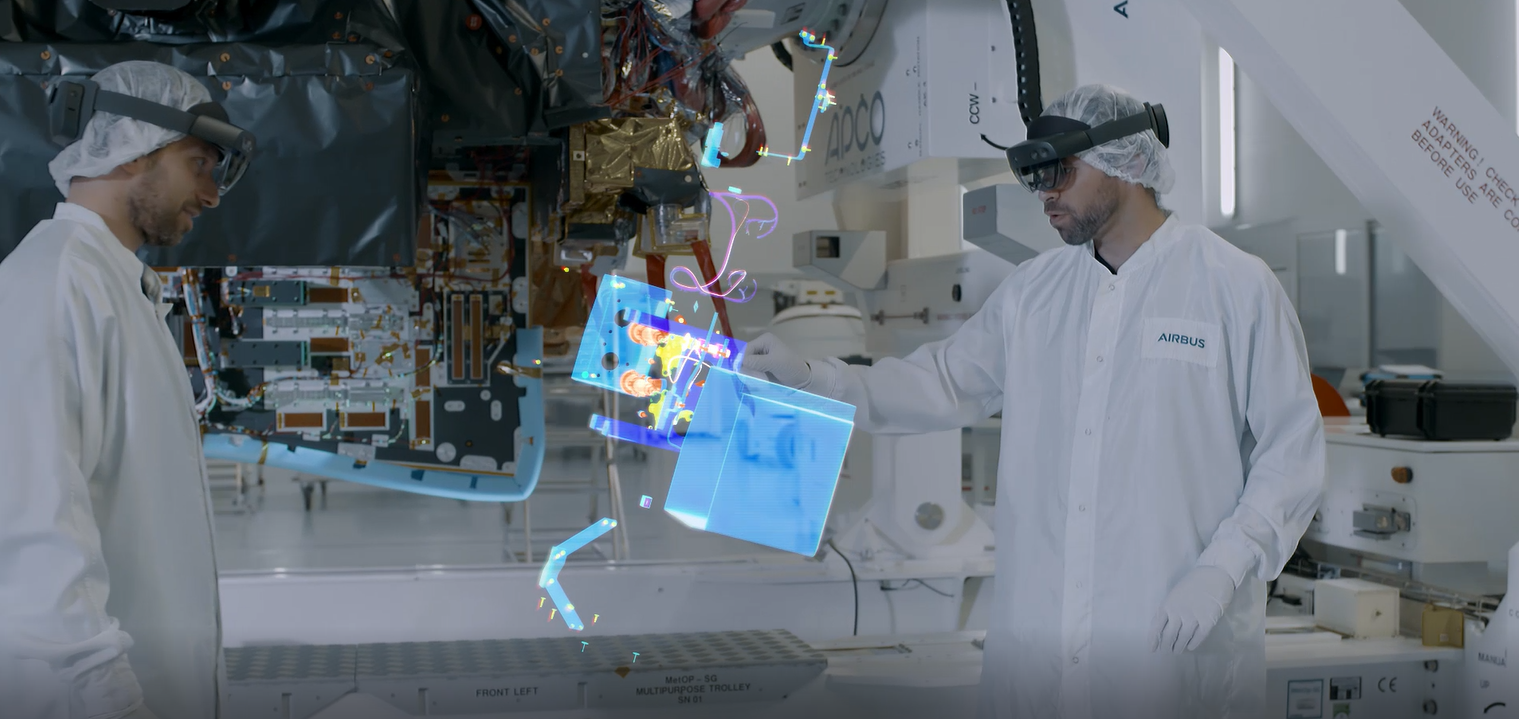
\includegraphics[scale=0.3]{Images/Estado del arte/ingenierosAirbus.png}
    \caption{Diseñadores de Airbus haciendo uso de las HoloLens 2.}
    \label{fig:ingenierosAirbusHololens2}
\end{figure}



La empresa ha detectado un total de 300 casos en los que la realidad mixta puede potenciar su trabajo, además, permite a los nuevos trabajadores aprender en un entorno virtual inmersivo (figura \ref{fig:ingenierosAirbusHololens2}) pudiendo así ver elementos en tres dimensiones desde cualquier ángulo, lo cual sería imposible sin este entorno.\\



El uso de esta tecnología mejora el rendimiento de los trabajadores ya que pueden trabajar de una forma más eficiente y ergonómica, de tal modo, la libertad de manos que ofrece unas gafas como las HoloLens2 de Microsoft aumenta la calidad y la seguridad del empleado.